\section{Overview}

Application of clustering algorithms to ground based lightning detection networks expands the real time global observations of lightning from strokes to flashes and strokes to thunderstorms.
Lightning detection networks, such as WWLLN or ENTLN, are then able to identify, locate, and analyze nearly every active thunderstorms within their operational range.
Global thunderstorm information allows for research into the climatological structures of thunderstorm behavior on large spatial and temporal scales.
Flash clustering allows for new network diagnostics, such as flash multiplicity and thunderstorm detection efficiency.

The DBSCAN algorithm is used to cluster strokes to flashes and thunderstorms for both the WWLLN and ENTLN.
Cross validation of the networks is performed with the located thunderstorms and comparisons of their inferred areas and duration.
Overall WWLLN detects 61\% of all ENTLN thunderstorm clusters and 80\% of thunderstorms larger than $10^3$~km$^2$.
In the reverse analysis, ENTLN detection of WWLLN thunderstorms, ENTLN detects 86\% of all WWLLN thunderstorms over North America.
On average WWLLN observes thunderstorm clusters lasting 10~minutes and spanning 66~km$^2$, ENTLN observes averages of 10~minutes and 60~km$^2$.
Within thunderstorms the average time between flashes is 21~seconds as seen by WWLLN and 10~seconds by ENTLN, with a strong dependence on season.
Clustering algorithms applied to lightning detection networks allow for a new range of analysis from thunderstorm effects, network performances, to the links between lightning and thunderstorms properties.

Lightning network detection efficiency is often measured in terms of relative stroke or flash performance through pair-wise comparisons of different systems.
For example comparing two ground based networks \citep{Abarca2010}, a ground based network with a satellite \citep{Rudlosky2013}, or a network to an actual ground truth such as rocket-and-wire triggered lightning \citep{Nag2011}.
In some cases, such as examining the global electric circuit (\citet{Hutchins2014}, Chapter~\ref{thesis:chapter:gec}), it is the location and properties of the thunderstorms generating the lightning that are important.
%% Add in some more thunderstorm important studies, see what cites Jacobson2006c
The thunderstorm detection efficiency for a lightning location system is then important in these applications, both the location, duration, and extent of the thunderstorm.

Within known thunderstorms the time between successive flashes can be used to examine further properties of the thunderstorm such as charging rate, controls on lightning strength, life cycle, and dynamics of the thunderstorm.
\citet{Zoghzoghy2013} examined the effect of the time between flashes as a measure of thunderstorm discharging in terms of the supression of future flashes.
\citet{Zipser1994} examined the relation between the flash rate in a thunderstorm with the updraft velocities, which in turn are controlled by the differential surface heating below the thunderstorm.
Only after considering and validating the performance of the lightning detection networks used can the effects of a flash be directly related to properties and behaviors of the parent thunderstorm.
Inferring thunderstorm properties based on the observed lightning flash rates can benefit regions with low availibility of direct or continuous observations (e.g. radar over oceans).

\section{Data}

%% Line about the detection efficiency?

The global WWLLN data will be used everywhere in this work unless specifically restricted to a given region, the ENTLN data will only be the North American subset of the data.
The data is from 2011 and 2012, with the exception of Section~\ref{thunderstorm:sec:interflash} which extends through June 2013.

\section{Methods}

Clustering the located strokes of both networks provides the thunderstorm and flash data.
The clustering is performed with the DBSCAN algorithm \citep{Ester1996, Kriegel2011a} following the application metholodgy discussed in Chapter~\ref{thesis:chapter:gec} \citep{Hutchins2014}.
DBSCAN is used over other clustering methods as it clusters based on the spatial and temporal distance between strokes with robust handling of noise (e.g. nearby thunderstorms).
The flash clustering uses the same algorithm as the thunderstorm clustering, with adjustment of the spatial and temporal clustering parameters.

For thunderstorms, WWLLN strokes are clustered together if they occur within $0.5^\circ$ and 18~minutes; for ENTLN it is $0.25^\circ$ and 15~minutes.
The tighter restraints on the ENTLN clustering stem from the higher density of strokes seen by ENTLN compared to WWLLN.
For flash clustering the strokes of both networks are clustered if they are within $0.12^\circ$ and 1~second of each other.
The 1~second timing is based on the natural inflection point observed in the WWLLN data (see Figure~\ref{thunderstorm:fig:interflash} in Section~\ref{thunderstorm:sec:interflash}).

The thunderstorm area is estimated by the best fit ellipse encapsulating all of the strokes in the cluster.
This will not be the areal extent of the thunderstorm system, rather just the electrified lightning region of the thunderstorm.
Similarly, thunderstorm duration is taken to be the time from the first stroke in a thunderstorm cluster to the last.
With these thunderstorm clustering parameters both networks observe similar average thunderstorm size and durations over North America.
WWLLN observes a median area and duration of 66 km$^2$ and 10~minutes, while ENTLN observes an average of 60 km$^2$ and 10 minutes.

A parameter used throughout this chapter is the time between successive strokes and flashes.
This interstroke time will refer to the time since the previous stroke in the parent thunderstorm cluster, while interflash time will refer to the time since the start of the previous flash in the thunderstorm cluster.

\section{Detection Efficiency}

The WWLLN thunderstorm detection efficiency is examined by comparing the located thunderstorm clusters with those located by ENTLN.
ENTLN does not have 100\% detection efficiency of strokes, it is used as a readily available baseline to compare to as a nominal ground truth for WWLLN.
Two thunderstorm clusters are considered to be matches if the convex hull of their constituent strokes overlap to within 5~km and $\pm5$~minutes.
Using a convex hull method requires at least three strokes in a thunderstorm for it be considered for a match; this creates an artifically lower detection efficiency for WWLLN for the cases where only 1 -- 2 strokes are detected in a thunderstorm.

Over the 2011 -- 2012 period in North America the average thunderstorm detection efficiency of WWLLN compared to ENTLN was 61\% while ENTLN has a detection efficiency of WWLLN of 86\%.
Similar to how detection efficiency varies with stroke strength, WWLLN has a higher detection efficiency of larger thunderstorms than smaller ones.
The spatial distribution of the detection efficiency is shown in Figure~\ref{thunderstorm:fig:deMap}.
In the southern regions, where there is typically higher thunderstorm activity, WWLLN has a detection efficiency above 70\%.
In regions with few thunderstorms (e.g. the West) there is a lower detection efficiency, possibly due to a lower detection efficiency of ENTLN in that region.

\begin{figure}[ht!]
   \centering
   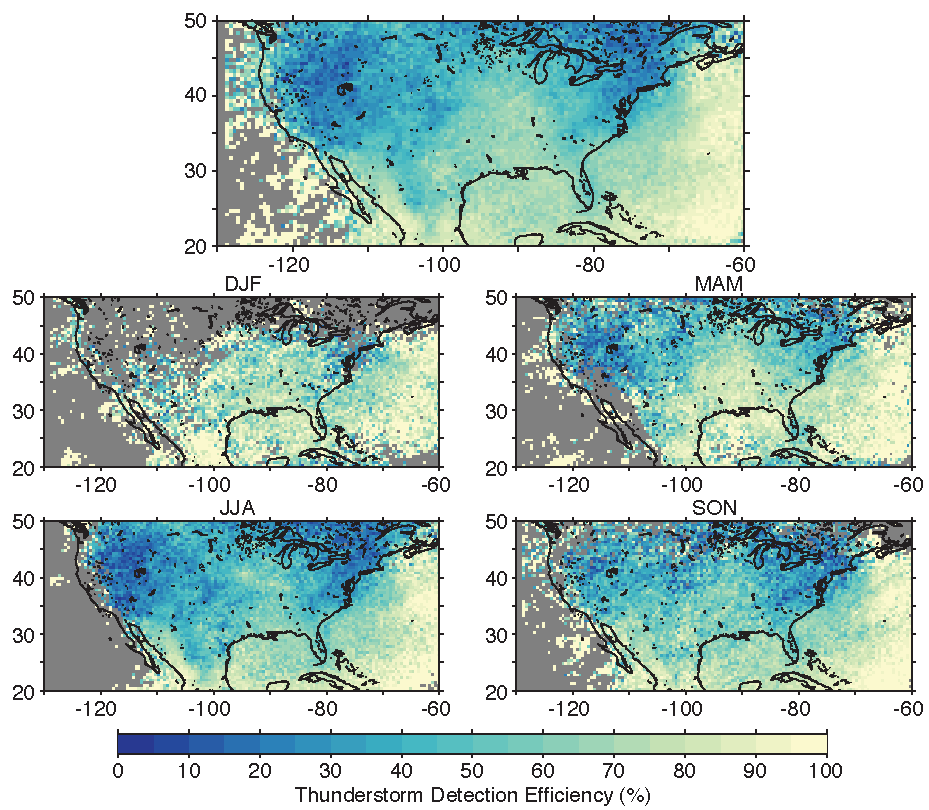
\includegraphics[scale=1]{thunderstorm/Figures/deMap.pdf}
   \caption{WWLLN detection efficiency of ENTLN thunderstorms over North America for 2011 -- 2012 (top panel), with each season broken out in the lower panels.}
   \label{thunderstorm:fig:deMap}
\end{figure}

The seasonal behavior shows a similar overall distribution of detection efficiency, with an overall increase in winter (DJF) and spring (MAM) compared to summer (JJA) and fall (SON).
A winter increase, 68\% compared to 56\% in summer, is tied to the decreased occurrence of thunderstorms during the cold season.
In all seasons WWLLN has the highest detection efficiency over the oceans.
Increased detection efficiency at the limits of the ETNLN detection range (e.g. in the center of the Atlantic Ocean) is convolved with the decreased efficiency of ENTLN and not solely an increase in the WWLLN detection efficiency.

The daily spatially averaged detection efficiency is shown in Figure~\ref{thunderstorm:fig:deDaily}.
Here the seasonal variation is  evident; the high levels of noise in the winter reflects the lower overall thunderstorm counts during these months.
Within the annual variation, the detection efficiency does not vary with thunderstorm area, size, or duration; there is only a constant overall change in detection efficiency for all thunderstorm types.

\begin{figure}[ht!]
   \centering
   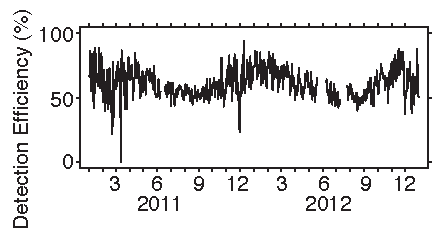
\includegraphics[scale=1]{thunderstorm/Figures/deDaily.pdf}
   \caption{Spatially averaged detection efficiency of ENTLN thunderstorms over North America.}
   \label{thunderstorm:fig:deDaily}
\end{figure}

The temporal distribution of thunderstorm detection efficiency can be split into different thunderstorm sizes (Figure~\ref{thunderstorm:fig:deBroken}a), total counts (Figure~\ref{thunderstorm:fig:deBroken}b), and durations (Figure~\ref{thunderstorm:fig:deBroken}c).
The daily detection efficiency increases for larger, productive, and longer thunderstorms.
For thunderstorms larger than $10^2$ km$^2$ the detection efficiency is 53\%, while for those larger than $10^3$ km$^2$ it is 80\%.
In a similar vein, thunderstorms with more than $10^2$~strokes are detected with 75\% efficiency and for more than $10^3$~strokes at 94\% efficiency.
Almost all thunderstorms observed are less than 1 hour in duration (Figure~\ref{thunderstorm:fig:deBroken}c, right), for those lasting more than 2 hours the detection efficiency increases to 93\%.


\begin{figure}[ht!]
   \centering
   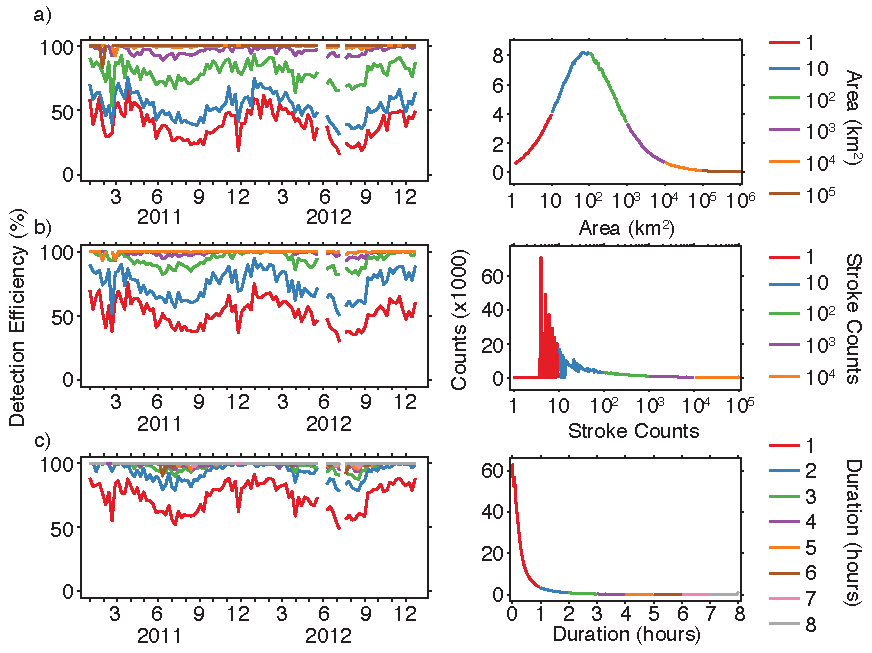
\includegraphics[scale=1]{thunderstorm/Figures/deBroken.pdf}
   \caption{Temporal variation in thunderstorm detection efficiency for different thunderstorm sizes: a) thunderstorm area, b) thunderstorm stroke counts, and c) thunderstorm duration.
           The distribution of thunderstorms for each parameter is shown in the right panels.}
   \label{thunderstorm:fig:deBroken}
\end{figure}

Removing the temporal variation demonstrates the trend of increasing detection efficiency for each thunderstorm parameter.
In Figure~\ref{thunderstorm:fig:deParameter} the black lines represent all thunderstorms and the colored lines split the thunderstorms by total counts detected by WWLLN in these thunderstorms.
Thunderstorm area, Figure~\ref{thunderstorm:fig:deParameter}a, shows a gradual increase in detection efficiency from 40\% to near 100\% efficiency above $10^3$ km$^2$; the total number of strokes does not have an independent effect from area of the thunderstorm.
Similarly the longer a thunderstorm is active the more likely it is to be detected by WWLLN, shown in Figure~\ref{thunderstorm:fig:deParameter}c.
Unlike area, this is convolved with the size and count of the thunderstorm: smaller thunderstorms have lower detection efficiency regardless of duration and larger thunderstorms are easier to detect.

\begin{figure}[ht!]
   \centering
   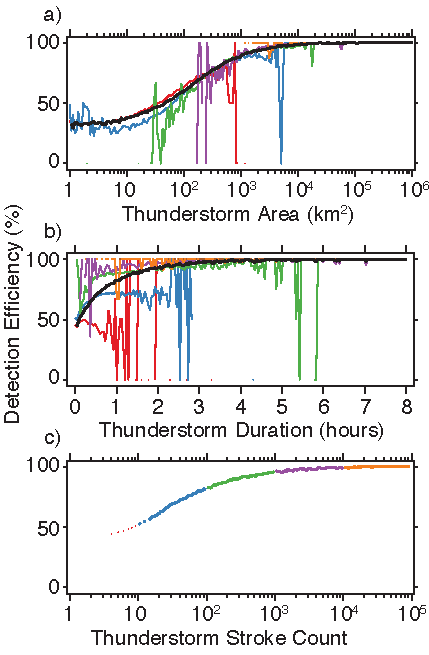
\includegraphics[scale=1]{thunderstorm/Figures/deParameter.pdf}
   \caption{Thunderstorm detection efficiency for different thunderstorm a) areas, b) stroke counts, and c) durations.
           Area and duration plots are shown with the overall average (black) and for different total stroke counts (colors) within the thunderstorms.}
   \label{thunderstorm:fig:deParameter}
\end{figure}

%% I don't like the first "shows" in this sentence.
Matching thunderstorms between the networks shows the overall performance of the networks but not how the characteristics of the thunderstorms differ between the two networks.
If the thunderstorm clusters are capturing intrinsic properties of the thunderstorms independent of the overall detection efficiency, then the properties should be same between both networks.
For example, if WWLLN measures a thunderstorm to have an area of 66~km$^2$ with 50~strokes and ENTLN measures an area of 60~km$^2$ with 200~strokes it can be said that both measure the actual estimated area of the thunderstorm cluster.
%% This needs to be better

The properties of the matched thunderstorm  between WWLLN and ENTLN can be directly compared for thunderstorm area and duration.
Density plots of the two networks estimation for each matched thunderstorm are shown in Figure~\ref{thunderstorm:fig:deSim}, where the counts in each bin are displayed on a log scale.
Each characteristics in Figure~\ref{thunderstorm:fig:deSim} shows a strong distribution along a single 1-to-1 line.
Area, Figure~\ref{thunderstorm:fig:deSim}a, has good agreement between both networks with 46\% of matches within $\pm25\%$ of each other; there is increased deviation for smaller thunderstorms compared to larger ones.
The WWLLN overestimation compared to ENTLN thunderstorm area may be caused by incorrect matches or accidental merging between two thunderstorm clusters.
The thunderstorm duration has the stronger relation of the two parameters, with 33\% of matches falling within $\pm25\%$ of the 1-to-1 line.
There is fairly good agreement between the two networks on thunderstorm properties despite the differences in overall detection efficiency.

\begin{figure}[ht!]
   \centering
   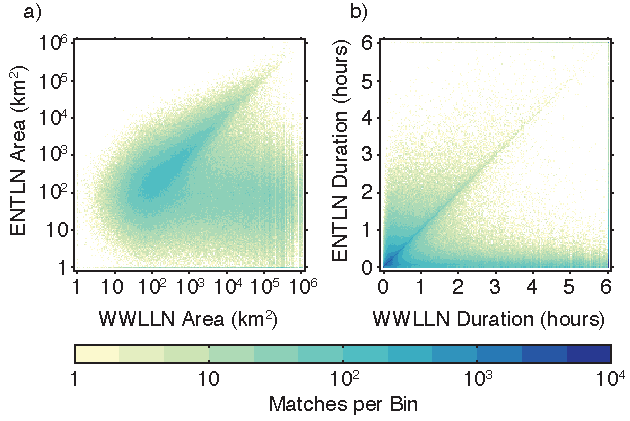
\includegraphics[scale=1]{thunderstorm/Figures/deSim.pdf}
   \caption{Thunderstorm comparison of matched thunderstorms for WWLLN and ENTLN for a) area and b) duration.
           Note: the density levels are on a log scale.}
   \label{thunderstorm:fig:deSim}
\end{figure}


The overall detection efficiency of WWLLN for ENTLN thunderstorms is lower than previous estimates of the networks thunderstorm detection performance, in this case it likely stems from only 67\% of WWLLN strokes clustered into thunderstorms.
The remaining 33\% of total strokes would increase the overall detection efficiency of thunderstorms for the cases where only 1 -- 2 WWLLN strokes match ENTLN thunderstorms.
In contrast ENTLN had 96\% of stroke clustered into thunderstorms due, in part, to the higher overall efficiency of the network.
The identified WWLLN thunderstorms exhibited similar characteristics to their corresponding ENTLN thunderstorms.

\section{Flash Clusters}
\label{thunderstorm:sec:interflash}

Within a thunderstorm cluster lightning detection networks are able to measure two additional properties: the interstroke and interflash timing.
The full WWLLN interstroke time, Figure~\ref{thunderstorm:fig:interflash}a, naturally shows two distinct peaks: one at 40~ms and another at 100~seconds with a natural inflection at 1~second.
With ENTLN the interstroke distribution does not show the same distinct peaks (Figure~\ref{thunderstorm:fig:interflash}c); because it is able to locate more strokes in each flash, the tail of the interstroke time distribution overlaps the interflash time distribution.
In the WWLLN interevent time distribution there is a spike of events near 10~$\mu$s caused by the same event recorded twice by the network, this also occurs less frequently with ENTLN.

\begin{figure}[ht!]
   \centering
   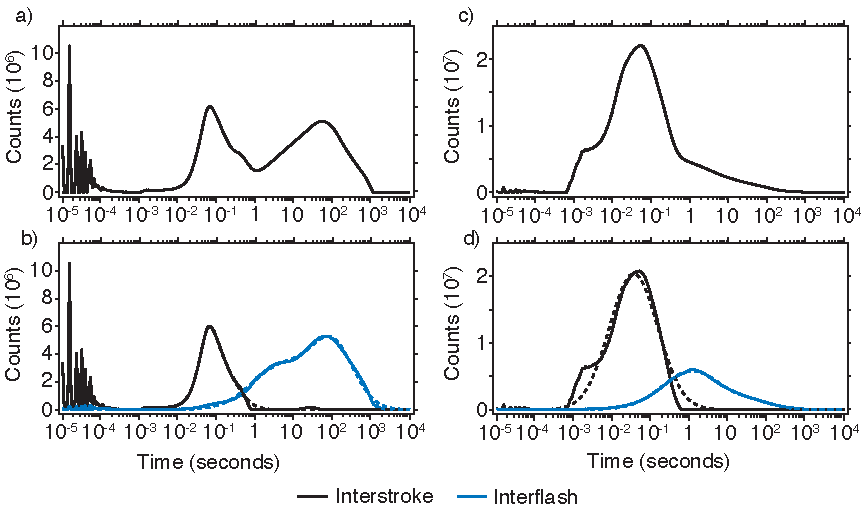
\includegraphics[scale=1]{thunderstorm/Figures/interflash.pdf}
   \caption{The interevent times for WWLLN (a) and ENTLN (c) and the interstroke (black) and interflash (blue) time distributions for WWLLN (b) and ENTLN (d).
           The dashed lines correspond to the best lognormal fits of the distributions.}
   \label{thunderstorm:fig:interflash}
\end{figure}

After the network events are clustered into flashes the time distributions can be split into the time between strokes in the same flash (black) and time between flashes (blue), shown in Figure~\ref{thunderstorm:fig:interflash}b and~\ref{thunderstorm:fig:interflash}d.
The stroke and flash distributions can be fit as lognormal distributions for each day of the year, an example set of fits is shown with the dashed lines in Figure~\ref{thunderstorm:fig:interflash}b and~\ref{thunderstorm:fig:interflash}d.
This fitting allows for the daily tracking of the interstroke (Figure~\ref{thunderstorm:fig:stability}a) and interflash (Figure~\ref{thunderstorm:fig:stability}b) times for both networks.
With WWLLN the global distributions (black) remain relatively centered at 71~ms and 100~seconds; over North America WWLLN averages (blue) are 60~ms for interstroke and 39~seconds for interflash times.
ENTLN (red) has lower daily averages of 53~ms and 17~seconds due to the higher detection efficiency.
The North American WWLLN distribution more closely matches the seasonal behavior present in the ENTLN distribution with a small offset in timing.

\begin{figure}[ht!]
   \centering
   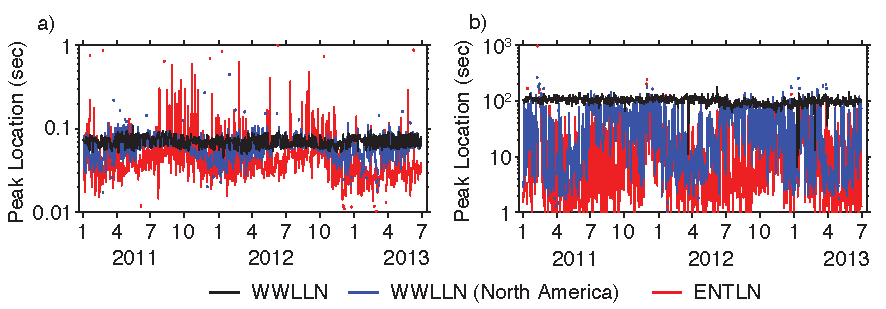
\includegraphics[scale=1]{thunderstorm/Figures/interflashStability.pdf}
   \caption{Peak of interstroke (a) and interflash (b) times for WWLLN (black), WWLLN over North America (blue), and ENTLN (red).
          Points beyond $2^{th}$ and $98^{th}$ percentiles shown as dots for WWLLN North America and ENTLN.}
   \label{thunderstorm:fig:stability}
\end{figure}

Directly comparing the time evolution of a thunderstorm will not work with thunderstorms of differing durations.
To account for this the thunderstorm life cycle is normalized by the duration of the thunderstorm.
Each thunderstorm is broken into 9 time segments where the first flash in the thunderstorm is at time~1 and the last flash at time~9.
With this normalization the average interflash time is found at each step for all thunderstorm clusters located by the two networks, shown in black in Figure~\ref{thunderstorm:fig:timerate}.
The interflash time can be seen to decrease to the center of a thunderstorms life cycle before increasing at the end, this is consistant with the known life cycle of a thunderstorm.
The interflash time for different energy (Figure~\ref{thunderstorm:fig:timerate}a) and absolute peak current (Figure~\ref{thunderstorm:fig:timerate}b) deciles are also shown.

\begin{figure}[ht!]
   \centering
   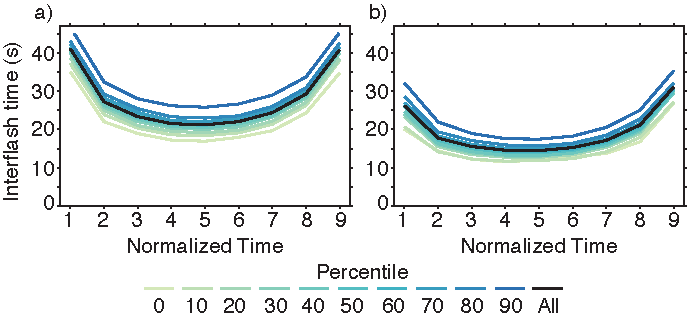
\includegraphics[scale=1]{thunderstorm/Figures/stormTimeRate.pdf}
   \caption{The interflash time for time-normalized thunderstorms for WWLLN (a) and ENTLN (b), with times shown for all flashes (black) and by stroke strength decile bins.
     WWLLN strength is divided by flash energy and ENTLN by absolute peak current.}
   \label{thunderstorm:fig:timerate}
\end{figure}

All flashes follow the same behavior, regardless of energy or peak current, however there are offsets in interflash time for different strength strokes.
As seen with WWLLN, Figure~\ref{thunderstorm:fig:timerate}a, the interflash time increases for more energetic strokes; for ENTLN, Figure~\ref{thunderstorm:fig:timerate}b, the interflash time increases for absolute peak current.
Between normalized time~1 and~5 the interflash time for the 90$^{th}$ percentile and above stroke strengths decreases by 9\% for WWLLN and 17\% for ENTLN compared to the median interflash time.
This shows that longer times between flashes results in stronger flashes; more charge separation can occur in the thunderstorm resulting in the stronger flashes.
In Figure~\ref{thunderstorm:fig:timerate} the separation between different flash strengths is consistant at all points in the thunderstorm life cycle.
It is not a constant offset but increases at the weaker stages of the thunderstorm (beginning and end) where longer time is necessary for a stronger flash, caused by a decreased charge separation rate.
The time between flashes is one of the main controlling factors in the strength of the resulting flash.
%% Speculation: over 9000

\section{Conclusion}

%% Discussion of the detection efficiency

When compared to ENTLN, WWLLN performs better when detecting large and active thunderstorm regions.
The lower performance for smaller thunderstorm clusters may be due to the cutoff in the clustering that requires at least 3 strokes for a cluster, removing 39\% of strokes from the analysis.
Including these strokes would lead to less robust matches between the networks and conflate a stroke to thunderstorm detection efficiency and the thunderstorm to thunderstorm detection efficiency.
For the thunderstorms WWLLN does detect, the characteristics of the thunderstorm are on par with those of ENTLN.

%% Discussion of flash clusters

On a global scale there is little change in the time between successive strokes and flashes within thunderstorms, but locally there are strong seasonal variations.
Both ENTLN and WWLLN observed the same seasonal variation in North America, with a small offset in their times based on the general detection efficiency differences in the networks.
The seasonal behavior shows a decrease in interflash times from the end of winter to the beginning of summer; thunderstorms in these times have higher flash rates compared to thunderstorms during the rest of the year.

The charging rate for thunderstorms evolves through the lifecycle of the thunderstorm, with the highest lighting flash rate during the middle of a thunderstorm.
The flash observed change in interflash time reflects the changes in the charging rate of the thunderstorm; the resulting flash stength depends on the charging rate and the total time charging between flashes.
If charging rate was constant with time than flash strength would be constant with interflash time through the life of a thunderstorm.
For a given charging rate the strength of the resulting flash depends on the time since the previous flash and the current thunderstorm convective activity.
